
We want to be able to integrate occurrence data into the Langevin model. For this, using a Bayesian framework is a possible solution. If the two processes has a common origin that they are conditioned on, we can use Bayes theorem to get information about that origin from both data sets. As we will see later the utilization distribution of the Langevin model fits this description. First though, we can demonstrate the implementation of a bayesian framework using just the track data. 


\section{The Bayesian Model}
The posterior distribution of parameters given the date is expressed as

$$
P(\theta | X) = \frac{p(x|\theta) \pi(\theta)}{\int_{\Omega_\theta} p(x|\theta)\pi(\theta)d\theta}
$$

Where $\theta$ is the set of parameters, $x$ is the data, $\pi$ is prior distribution of the parameters, and $\Omega_\theta$ is the parameter space. The prior distribution of the parameters represents the modellers beliefs about the distribution of the parameters prior to having information from the data. Broadly speaking there are two ways of defining a prior distribution: using an informed prior and using an uninformed prior. informed priors incorporate knowledge from people which is then
updated by the data. uninformed priors on the other hand, try to spread out
the distribution of the priors as much as possible, to give a prior containing the least amount of bias. This can be accomplished by for example using a normal distribution with very high variance. 

From the Euler approximation we have an approximate expression for the likelihood as 

$$
P(\textbf{X} = \textbf{x}|\theta) = \prod_{i=1}^M \prod_{j=1}^{m_i} q_{\Delta_i}(\textbf{x}_{ij}|\textbf{x}_{i(j-1)}, \beta, \gamma)
$$

where $M$ is the number of tracks, $m_i$ is the number of data points in each track and $\textbf{x}_{ij}$ is the j-th data point in the i-th track and $\Delta_{ij}$ is the time-difference between $x_{ij}$ and $x_{i(j-1)}$. $q_{\Delta}$ are the normally distributed transition probabilities with mean $X_{i(j-1)} + \gamma^2\Delta_{ij}(\sum_{k = 1}^j \beta_k \nabla c_k(x_{i(j-1)}))$ and variance $\gamma^2\Delta_{ij}$. To demonstrate the model we will be using data simulated from ten tracks, with a step interval of $\Delta = 0.02$ and a maximum time of $5000$, using the same method to simulate data as for figure \ref{fig:example_1_estimates}.

Usually it is hard to make inferences directly from the posterior distribution because in most cases it is difficult to compute the integral meant to normalize the distribution. Instead we can make inferences about the distribution using the Markov chain Monte Carlo methods (MCMC), which constructs a Markov-chain whose stationary distribution is equal to the target distribution that we are trying to sample from. Alternatively the method INLA (INSERT CITATION) uses ...

\section{Using MCMC}

To  be able to construct our Markov chain the first step will have to be to choose a kernel density for the random walk. The normal distribution is a good choice for this because it is symmetric, meaning it does not have a bias toward any direction, and its tails stretch to both infinities, meaning all values can in theory be reached in one step. The variance of the random walk proposal determines the mixing of the Markov chain. having a too small variance Will result in small steps. These might get accepted more often, but the parameter space is explored more slowly, leading to less mixing and slower convergence. On the opposite end the variance might be to big meaning the proposed values rarely get accepted. It is recommended that the acceptance rate should be around 20\% to 50\% to have a balance between accepting values and exploring the state space(INSERT CITATION). 


For this example we start with a variance of $\sigma^2 = 0.0001$, and starting parameters $\beta_1 = \beta_2 = \beta_3 = 0$ and $\gamma^2 = 1$. 

\begin{figure}[H]
    \centering
    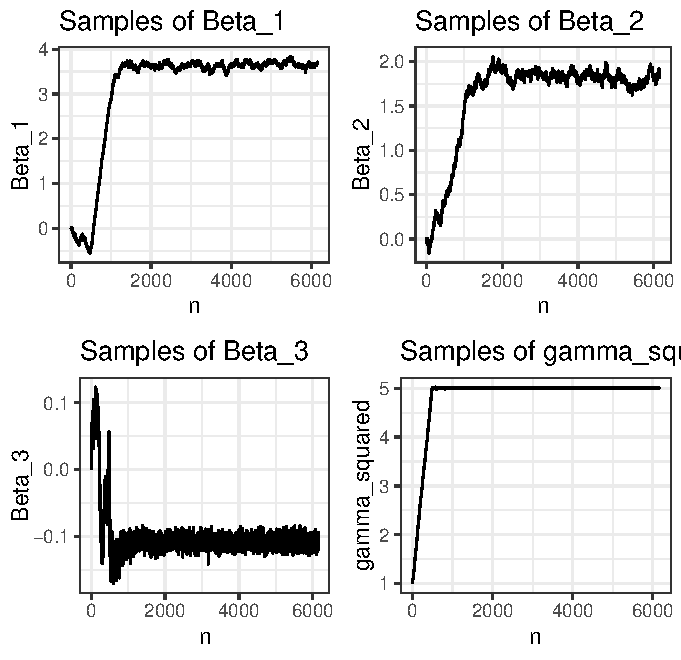
\includegraphics[width=\linewidth]{Images/ch3/MCMC_sample1_plot.pdf}
    \caption[MCMC1]{trace plots samples from Markov chain simulating posterior distribution of parameters using track data}
    \label{fig:MCMC1_plot}
\end{figure}

Figure \ref{fig:MCMC1_plot} shows that the Markov chain converges quickly. After $2000$ samples the chain appears to have reached stationarity. after this the mean of the samples are $\beta_1 = 3.61$, $\beta_2 = 1.81$, $\beta_3 = -0.11$ and $\gamma^2 = 5.0$. The overall average acceptance rate of the chain is $\alpha = 0.277$. The covariance matrix of the sample after the burn-in period was

$$
\begin{pmatrix}
    2.766298e-02 & 1.164617e-02 & 1.650621e-04 & -4.333012e-05 \\
    1.164617e-02 & 1.179554e-02 & -2708569e-05 & -2366656e-05 \\
    1.650631e-04 & -2.708569e-05 & 6.495500e-05 & -1108711e-06 \\
    -4.333012e-05 & -2.366656e-05 & -1.108711e-06 & 1.329572e-05 
\end{pmatrix}
$$


The Markov chain can be improved upon by creating a new Markov chain where the proposal has a covariance matrix which is the covariance of the samples after the burn-in period. This way the covariance with low variance can have small steps, while the covariance with large variance can have large ones. In addition the covariance structure between the parameters is accounted for in the steps of the Markov chain, giving a chain that mixes more efficiently. Figure \ref{fig:MCMC2_plot} shows a Markov chain constructed this way with starting values equal to the mean of the previous chain after the burn-in period.


\begin{figure}[H]
    \centering
    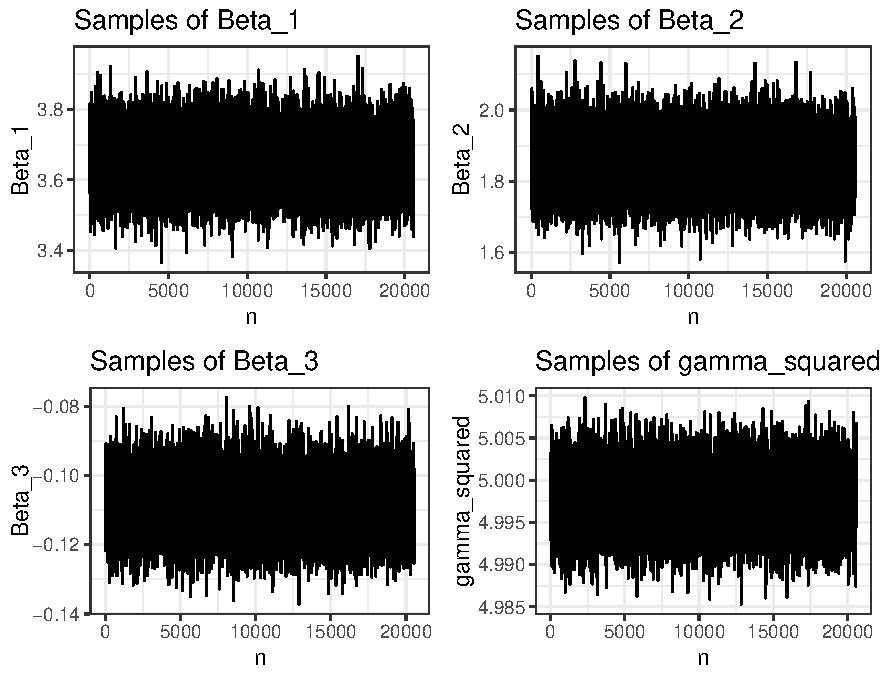
\includegraphics[width=\linewidth]{Images/ch3/MCMC_sample2_plot.pdf}
    \caption[MCMC1]{trace plots of samples from Markov chain simulating posterior distribution of parameters using track data}
    \label{fig:MCMC2_plot}
\end{figure}

There are multiple ways of assessing the quality of the sample. Firstly we can look at the trace plot. If the Markov chain has converged, the trace plot should have no large-scale drifts. As we see from Figure \ref{fig:MCMC2_plot}, this is the case for the Markov chain sample. we can also judge the quality of the sample by looking at the auto correlation of the sample defined as

$$
\hat{\rho(k)} \approx \frac{\sum_{i=1}^{N-k}(x_i-\Bar{x})(x_{i+k}-\Bar{x})}{\sum_{i=1}^N(x_i-\Bar{x})^2}
$$

For a sufficiently large N. The auto correlation function defines the correlation between different points of the samples at a certain lag $k$. Using this we can see how well the chain mixes. If the auto correlation function decreases slowly with the lag, it is a sign that the Markov chain mixes slowly. 

\begin{figure}[H]
    \centering
    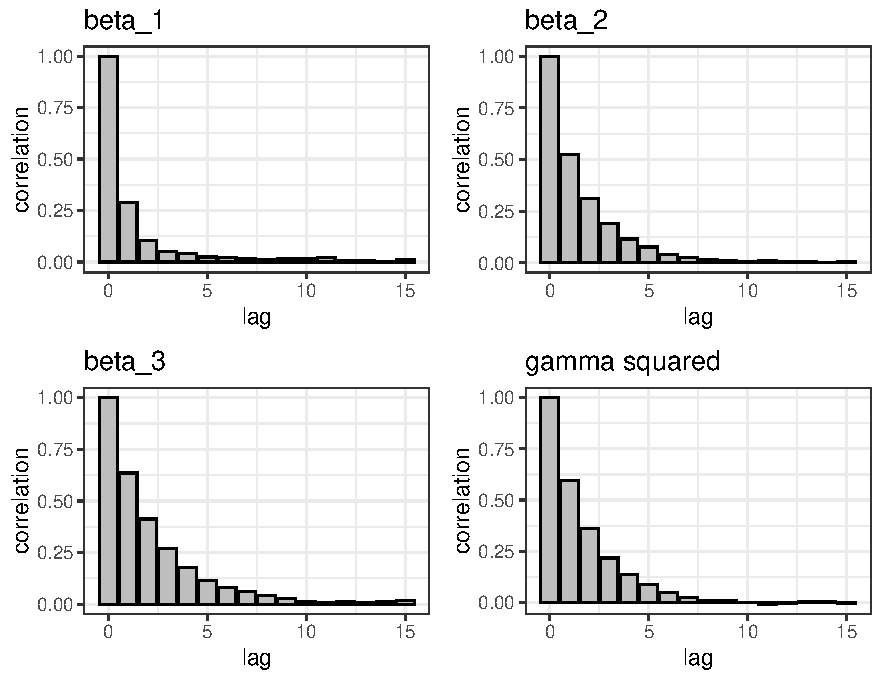
\includegraphics[width=\linewidth]{Images/ch3/MCMC_sample2_autocorrplot.pdf}
    \caption[MCMC1]{auto correlation functions of Markov chain samples.}
    \label{fig:MCMC2_autocorr}
\end{figure}

Figure \ref{fig:MCMC2_autocorr} shows that the auto correlation functions of the samples decreases rapidly, which suggests that the mixing of the chain is good. From the auto correlation function we can also compute the effective sample size \cite{kass_markov_1998}

$$
ESS = \frac{N}{\tau} , \ \tau = 1 + 2\sum_{k=1}^\infty \hat{\rho}(k)
$$

As the name suggests, this gives an indication of the size of the sample if it had had independent observations. We can use the R library "coda" to calculate this value. Doing this gives that the effective sample size of the sample is 10076.89 independent samples. Since the effective size of the sample is large we can uses it to make inferences about the parameters of the model. 


\begin{figure}[H]
    \centering
    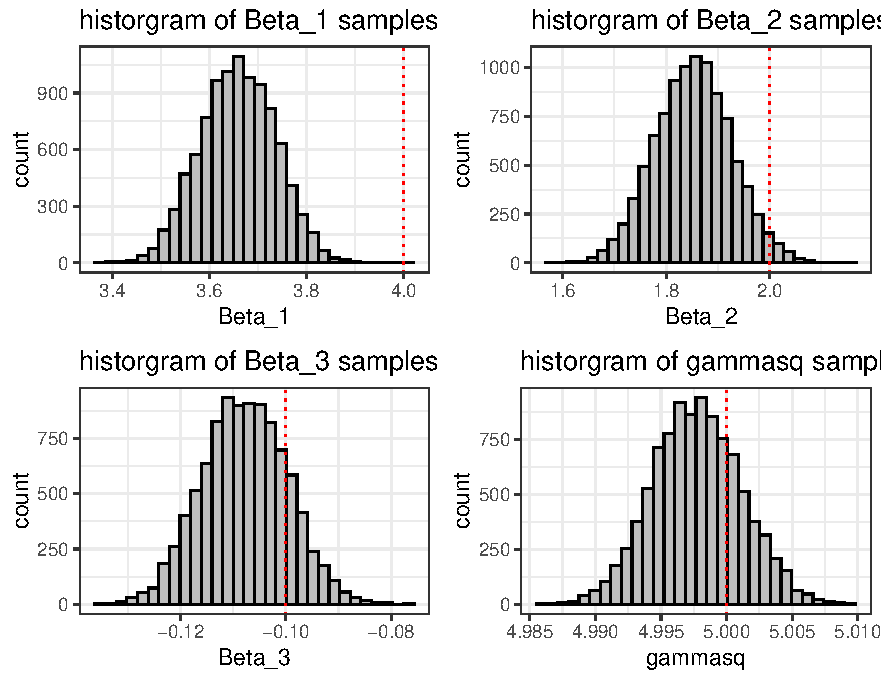
\includegraphics[width=\linewidth]{Images/ch3/MCMC_sample2_hist.pdf}
    \caption[MCMC1]{histograms of Markov chain samples. The true value of the parameters is shown with a red dotted line.}
    \label{fig:MCMC2_hist}
\end{figure}

Figure \ref{fig:MCMC2_hist} shows histograms of the sampled parameters, with the true value of the parameters represented by a red dotted line. From the histograms we see that, as demonstrated earlier, the values are underestimated somewhat. For $\beta_1$ and $\beta_2$ this underestimation is large, and most of the sampled values are smaller than the true value, but for $\gamma^2$ the difference is not as large. For $\beta_3$ the estimated effect is actually larger than the true value. Taking the mean of the samples we get the etsimates $\hat{\beta_1} = 3.658661$, $\hat{\beta_2} = 1.853568$, $\hat{\beta_3} = -0.1080579$, $\hat{\gamma^2} = 4.997666$.